\section*{8.3 The Symmetric QR Algorithm} %{{{1

The symmetric QR-iteration can be made very efficient in two ways.
\begin{enumerate}[(a):]
	\item First, an orthogonal $U_0$ is calculated such that $U_0^T A U = T$ is tridiagonal.
	With this reduction the iterates $T_k$ of Alg. \ref{algQRIterSimple} is also tridiagonal,
	meaning that each iteration is reduced to $\mathcal O(n^2)$ flops.
	\item The idea of shifts are introduces, boosting the convergence from linear to cubic.
\end{enumerate} 

\subsection*{8.3.1 Reduction to Tridiagonal Form}%{{{2

If $A$ is symmetric, then it is possible to find an orthogonal $Q$ s.t. $Q^TAQ=T$ is tridiagonal.
This is called the tridiagonal decomposition. Note that $T$ is symmetric since
$T^T = (Q^TAQ)^T = T$.
Below it is discussed how the tridiagonal decomposition can be computed using Householder matrices.

A Householder matrix describes a reflection in the hyper surface $\text{span}(v_\bot)$, and can be 
written on the general form $H = I - 2{vv^T}/{v^Tv}$. This is a reflection since, for a general 
vector $x$, $Hx=x - 2({v^Tx}/{v^Tv})v$. It is always possible to find a Householder vector $v$, s.t. 
$Hx\propto e_1$. Numerically this is an $\mathcal O(n)$ operation.

For a $n\times n$ symmetric matrix $A$, the Householder reduction is found in a stepwise process
\begin{enumerate}[(a):]
	\item Find the $n-1\times n-1$ Householder matrix $H_1$ s.t. $H_1A(2:n,1)\propto e_1^{(n-1)}$
	\item Find the $n-2\times n-2$ Householder matrix $H_2$ s.t. $H_1A(3:n,1)\propto e_1^{(n-2)}$
	\item $\dots$
	\item Find the $2\times 2$ Householder matrix $H_{n-2}$ s.t. $H_1A(n-1:n,1)\propto e_1^{(2)}$
	\item Assume that
	\begin{equation}
	\tilde H_k =	
	\begin{matrix}
		\\	
		\smatrix{I & 0 \\ 0 & H_{k}}
		&
		\begin{matrix}		
			k \\ n-k
		\end{matrix}
		\\
		\begin{matrix}		
			k & n-k
		\end{matrix}
	\end{matrix}
	\end{equation}
	for $k \in \{1,2,3,\dots,n-2\}$. Now
	\begin{align}
		&\tilde H_{n-2} \tilde H_{n-1} \dots \tilde H_1 A = \text{Matrix on upper Hessenberg form.}\\
		&\tilde H_{n-2} \tilde H_{n-1} \dots \tilde H_1 A 
			\tilde H_{1} \tilde H_{2} \dots \tilde H_{n-2} = T = \text{Tridiagonal matrix}
	\end{align}
Note, from the definition of $H_k$, that $H_k=H_k^T$. The last equation above is easy
to understand if the individual operations $H_1AH_1$ is inspected. If this is done, it is also easy 
to see why the Householder reduction is unable to take $A$ to the diagonal form.
\end{enumerate}
The Householder reduction involves $4n^3/3$ flops if the symmetries of $A$ is exploited.

%}}}2

\subsection*{8.3.2 Properties of the Tridiagonal Decomposition}%{{{2

Two theorems about the tridiagonal decomposition are stated below.
\begin{definition}(Krylov Matrix):
A Krylov Matrix is a matrix on the form
\begin{equation}
	K(A,v,k) = [v, Av, A^2v,\dots,A^{k-1}v],\, A\in\mathbb R^{n\times n},\,v\in\mathbb R^n.
\end{equation}
\end{definition}
%
\begin{theorem}():
If $Q^TAQ=T$ is the tridiagonal decomposition of the symmetric matrix $A\in \mathbb R^{n\times n}$,
then $Q^TK(A, Q(:,1),n) =R$ is upper triangular.
%
If $R$ is nonsingular then $T$ is unreduced
\footnote{The tridiagonal decomposition is reduced if one of the sub/super-diagonal entries is zero.}
. If $R$ is singular and $k$ is the smallest index 
where $R_{kk}=0$ then $k$ is the smallest index where $T_{k,k-1}=0$. 
\end{theorem}
%
\begin{theorem}(The implicit Q Theorem):
Suppose $Q=(q_1,q_2,\dots,q_n)$ and $V=(v_1,v_2,\dots,v_n)$ are orthogonal matrices with the property
that both $Q^TAQ=T$ and $V^TAV=S$ are tridiagonal where $A\in\mathbb R^{n\times n}$ is symmetric.
Let $k$ denote the smallest index where $T_{k+1,k}=0$, with the convention that $k=n$ is $T$ is 
unreduced. If $v_1=q_1$ than $v_i=\pm q_i$ and $T_{i,i-1} = S_{i,i-1}$ for $i=2:k$. Moreover, if
$k<n$, then $S_{k+1,k}=0$.
\begin{equation}
.
\end{equation}
\end{theorem}

%}}}2

\subsection*{8.3.3 The QR Iteration and Tridiagonal Matrices}%{{{2

Here four facts about the QR-iteration and tridiagonal matrices are stated.
%
\begin{enumerate}[(a):]
\item Preservation of form: If $T=QR$ is the QR-factorization of a symmetric tridiagonal matrix
$T\in\mathbb R^{n\times n}$, then $Q$ has lower bandwidth 1 and $R$ has upper bandwidth 2, 
and it follows that
\begin{equation}
	T_+ = RQ = Q^T(QR)Q = Q^TTQ
\end{equation}
is also symmetric and tridiagonal.
\item Shifts: If $s\in\mathbb R$ and $T-sI=QR$ is the QR-factorization, then
\begin{equation}
	T_+ = RQ + sI =Q^TTQ.
\end{equation}
Is also tridiagonal. This is called the shifted $QR$ step.
\item Perfect shifts: If $T$ is unreduced, then the first $n-1$ columns of $T-sI$ are independent 
regardless of $s$ Thus, if $s\in\lambda(T)$ and $QR=T-sI$ is a QR-factorization, then $r_{nn}=0$
and the last column of $T_+=RQ-sI$ equals $sI(:,n)=se_n$.
\item Cost: If $T\in\mathbb R^{n\times n}$ is tridiagonal, then it's QR factorization can be computed
by applying a sequence of $n-1$ Givens rotations which requires $\mathcal O(n)$ flops.
If the rotations are to be accumulated, then $\mathcal O(n^2)$ flops are required.
The algorithm is listed in Alg. \ref{algQRFacTridiagMat}.
\end{enumerate}
%
%
\begin{algo}
{
%
	(QR factorization of a tridiagonal matrix):
%
}\\
\textbf{Input: }
{
%
	\\The symmetric and tridiagonal matrix $T\in\mathbb R^{n\times n}$.
%
}\\
\textbf{Output: }
{
%
	\\$Q$ if the rotations are accumulated.
	\\$R$ as $T$?.
%
}\\
\line(1,0){150}
\begin{algorithmic}
%
\For{k=1:n-n}
	\State{$[c,s]=givens(T_{kk},T_{k+1,k})$}
	\State{$m=\text{min}(k+2,n)$}
	\State{$T(k:k+1,k:m) = \smatrix{c&s\\-s&c}^TT(k:k+1,k:m)$}
\EndFor{}
%
\end{algorithmic}
\label{algQRFacTridiagMat}
\line(1,0){150}
\end{algo}
%\end{algorithm} 
%

%}}}2

\subsection*{8.3.4 Explicit Single Shift QR Iteration}%{{{2

If $s$ is close to an eigenvalue then we suspect that $T_{n,n-1}$ will be small after a $QR$ step
with shift $s$. This can be made very intuitive if we remember from the QR algorithm 
that the convergence of the eigenvectors $v_1,\dots,v_n$ ($v_i=Qe_i$) converges with a rate 
proportional to $|\lambda_i/\lambda_{i+1}|$.
The shift shifts the eigenvalues with $-s$, and if 
$s\approx\lambda_{i+1}$, we increase the separation 
between the eigenvalues and thereby accelerate the convergence. 

Below follows a small example to show why the single shift 
speeds up the convergence of the $n$'th eigenvector.
This example is in the context of the orthogonal iteration algorithm, which is simply an
alternative formulation of the $QR$-algorithm. (?? Ask Morten)
We write $T$ as the spectral decomposition
\begin{equation}
	T = \sum_i \lambda_i v_i^Tv_i
\end{equation}
We introduce the shifted matrix $\tilde A = A - sI$, where all eigenvectors are shifted by $s$ while
the eigenvectors are the same. 
The multiplication of the $i$'th row of $Q_k$ ($q^{k}_i=Q_ke_i$) yields
\begin{equation}
	Tq^k_i = \sum_i \lambda_i (v_i^Tq^k_i) v_i
\end{equation}
where all $q^k_i$'s will be rotated in the direction of the eigenvector with the shifted 
eigenvector with the eigenvalue with the largest modulo. 
In the process of the QR factorization of $TQ_k\to Q_{k+1}R_{k+1}$, the following happens:
$q^{k+1}_1\propto q^k_1$, but
$q^{k+1}_2$, is set to be orthogonal to $q_1$, and will therefore tend against the eigenvector 
with the eigenvalue with the second largest modulo. And so it goes for $q^{k+1}_3,q^{k+1}_4,\dots$.
If $s\approx\lambda_n$, all $q^{k+1}_i$ will have a small component of $v_n$ except to $q^{k+1}_n$
which is set to be orthogonal to $q^{k+1}_i,i\neq n$, and therefor will have a large component 
of $v_n$. Now $I\lambda$ must be added to $T$ to reset the eigenvalue to it's correct value.

A reasonable guess for the $n$'th eigenvalue is simply $s=a_n$ since $T$ already is close to it's
diagonal form. An other possibility is to choose $s$ to be the eigenvalue of the block.
\begin{equation}
	\smatrix{a_{n-1}&b_{n-1}\\b_{n-1}&a_n}
\end{equation}  
which is 
\begin{equation}
	s=a_n+d-\sign{}(d)\sqrt{d^2+b_{n-1}^2},\,(a_{n-1}-a_n)/2.
\end{equation}
This is called the Wilkinson shift.
%
Both strategies are known to give a cubic convergence.
%
%
\begin{algo}
{
%
	(Explicit Single Shift QR):
%
}\\
\textbf{Input: }
{
%
	\\The symmetric and tridiagonal matrix $T\in\mathbb R^{n\times n}$.
%
}\\
\textbf{Output: }
{
%
	\\$T$ as the Shur decomposition.
	\\$Q$ where $Qe_i$ is the $i$'th eigenvector.
%
}\\
\line(1,0){150}
\begin{algorithmic}
%
\State{$T=U_0^TAU_0$}
\For{k=1,2,\dots}
	\State{Determine the shift $s\in\mathbb R$}
	\State{$UR\gets T-sI$ (QR-factorization)}
	\State{$T\gets RU+sI$}
\EndFor{}
%
\end{algorithmic}
\label{algQRSingleShiflExplicit}
\line(1,0){150}
\end{algo}
%\end{algorithm} 
%


%}}}2

\subsection*{8.3.5 Implicit Single Shift Version}%{{{2

It is possible to execute the transition from $T$ to $T_+$ without explicitly forming the matrix
$T-sI$. This is advantageous when the shift is much larger than some of the $a_i$. 
\footnote{Why??}

Note that the explicitly shifted QR-iteration is equivalent to the transformation
\begin{align}
	T_+ = RU + sI = U^TTU \text{ where }
	UR = T + sI \text{ (QR-transform)}.
\end{align}

We want to form a matrix $Z$ which is a product of givens transformations
\begin{align}
	&Z = Z_{n-1}Z_{n-2}\dots Z_{1}, \notag\\ 
	&Z_i = 
		\smatrix{ 
				I^{i-1\times i-1} 	& 0 	& 0 \\ 
				0 					& G_i 	& 0 \\ 
				0 					& 0 	& I^{n-i-2\times n-i-2}}, \notag\\
	&G_i = \smatrix{cos(\theta_i) & \sin(\theta_i) \\ -\sin(\theta_i) & \cos(\theta_i)}
\end{align}
where the first column of $Z$ is equal to the first column of $U$.
Also note that $Ze_1 = Z_1e_1$
According to the implicit Q theorem, when $Ue_1=Ze_1$, and both $U^TTU$ and $Z^TTZ$ are
tridiagonal, then $U^TTU$ and $Z^TTZ$ are essentially equal. Here, essentially equal means that
$U^TTU = D(Z^TTZ)D$ where $D = \diag(\pm1,\pm1,\dots,\pm1)$, meaning that the off diagonal 
elements $b_i$ of the two matrices can have different signs. 
However, since $D$ is an unitary transform, the eigenvalues will be the same, meaning 
that the two approaches introduce the same shift $s$.

To set $Ze_1=Ue_1$ we must find a $\theta_1$ such that
\begin{equation}
	G_1 
	\smatrix{ T_{11}-s \\ T_{21} } \propto \smatrix{ 1 \\ 0} = 
	\smatrix{ \cos(\theta_1) & \sin(\theta_1) \\ -\sin(\theta_1) & \cos(\theta_1) } 
	\smatrix{ T_{11}-s \\ T_{21} } \propto \smatrix{ 1 \\ 0} \label{eq835}. 
\end{equation}
Note that 
\begin{equation}
	QRe_1 = \smatrix{T_{11}-s\\T_{21}\\0\\0\\ \vdots} 
	\Rightarrow Qe_1 \propto  \smatrix{T_{11}-s\\T_{21} \\0\\0\\ \vdots}
\end{equation}
since $R$ is upper triangular. Then
\begin{equation}
	G_1 \propto  \smatrix{T_{11}-s & -T_{21} \\ T_{21} & T_{11}-s}
\end{equation}
Since both $Z$ and $U$ is orthogonal, the proportionality of Eq. \eqref{eq835} implies that 
the first column of $Z$ and $U$ is equal.

The next step is to show how $G_i,\,i>1$ can be constructed such that $Z^TTZ$ is tridiagonal.
First, look at this example where $T$ is an $5\times 5$ matrix.
\begin{equation}
	Z_1 ^T T Z_1= 
\smatrix
{
\times 	& \times & \times & 0 & 0   \\
\times 	& \times & \times & 0 & 0   \\
\times 	& \times & \times & \times & 0   \\
0 & 0 & \times & \times & \times     \\
0 & 0 & 0 & \times & \times    \\
}
.
\end{equation}
$Z_2$ is constructed s.t.
\begin{equation}
	Z_2^TZ_1 ^T T Z_1 Z_2 = 
\smatrix
{
\times 	& \times & 0 & 0 & 0   \\
\times 	& \times & \times & \times & 0   \\
0 	& \times & \times & \times & 0    \\
0 & \times & \times & \times & \times   \\
0 & 0 & 0 & \times & \times  \\
}
.
\end{equation}
$Z_3$ is constructed s.t.
\begin{equation}
	Z_3^TZ_2^TZ_1 ^T T Z_1 Z_2 Z_3 = 
\smatrix
{
\times 	& \times & 0 & 0 & 0   \\
\times 	& \times & \times & 0 & 0   \\
0 	& \times & \times & \times & \times    \\
0 & 0 & \times & \times & \times   \\
0 & 0 & \times & \times & \times  \\
}
.
\end{equation}
And finally, $Z_4$ is constructed s.t.
\begin{equation}
	Z_4^TZ_3^TZ_2^TZ_1 ^T T Z_1 Z_2 Z_3 Z_4= 
\smatrix
{
\times 	& \times & 0 & 0 & 0   \\
\times 	& \times & \times & 0 & 0   \\
0 	& \times & \times & \times & 0    \\
0 & 0 & \times & \times & \times   \\
0 & 0 & 0 & \times & \times  \\
}
.
\end{equation}
The $G_i$'s can be found by solving the following equation
\begin{align}
\smatrix{
1 & 0 & 0 & 0 \\
0 & c & s & 0 \\
0 & -s & c & 0 \\
0 & 0 & 0 & 1 
}
\smatrix{
a_i& b_i & z_i & 0 \\
b_i & a_p & b_p & 0 \\
z_i & b_p & a_q & b_p \\
0 & 0 & b_q & a_r 
}
\smatrix{
1 & 0 & 0 & 0 \\
0 & c & s & 0 \\
0 & -s & c & 0 \\
0 & 0 & 0 & 1 
}
=
\smatrix{
a_i& b_i & 0 & 0 \\
b_i & a_p & b_p & z_p \\
0 & b_p & a_q & b_p \\
0 & z_p & b_q & a_r 
}
\end{align}
where $(p,q,r)=(i+1, i+2, i+3)$. We simply need to find a $b_is+z_ic = 0$
and then to explicitly do the transform. (involves approx. 26 flops).
$G_i$ can be written 
\begin{align}
	G_i = \frac1{N}\smatrix{ 1 & \frac{z_i}{b_i} \\ -\frac{z_i}{b_i} & 1 }
	\text{ where } N = \left[\frac{z_i}{b_i}\right]^2+1.
\end{align}

\begin{algo}
{
%
	(Implicit symmetric QR-step With Wilkinson Shift):
%
}\\
\textbf{Input: }
{
%
	\\The symmetric and tridiagonal matrix $T\in\mathbb R^{n\times n}$.
%
}\\
\textbf{Output: }
{
%
	\\$T$ is overwritten with $T_+Z^TTZ$.
%
}\\
\line(1,0){150}
\begin{algorithmic}
%
\State{$d\gets (T_{n-1,n-1}-t_{nn})/2$}
\State{$\mu \gets (T_{nn} - T^2_{n,n-1})/(d+\text{sign}(d)\sqrt{d^2+T^2{n,n-1}})$}
\State{$x \gets T_{11}-\mu$}
\State{$z \gets T_{21}$}
\For{k=1:n-1}
	\State{$[c,s] \gets \text{givens}(x,z)$}
	\State{$T \gets G_k^TTG_k$}
	\If{$k<n-1$}
		\State{$x\gets T_{k-1,k}$}
		\State{$z\gets T_{k-2,k}$}
	\EndIf{}
\EndFor{}
%
\end{algorithmic}
\label{algImplicitQRStep}
\line(1,0){150}
\end{algo}
%
This algorithm requires about $30n$ flops to find $T_+$, and an other $6n^2$ if the orthogonal matrix
$Q$ is to be overwritten with $QZ_1\dots Z_{n-1}$.
%
\begin{algo}
{
%
	(Symmetric QR Algorithm):
%
}\\
\textbf{Input: }
{
%
	\\The symmetric matrix $T\in\mathbb R^{n\times n}$.
%
}\\
\textbf{Output: }
{
%
	\\$T$ as the Shur decomposition.
%
}\\
\line(1,0){150}
\begin{algorithmic}
%
\State{Compute the tridiagonalization $T\gets A$:}
	\State{\hspace{4mm} $T=(P_1\dots P_n-2)^TA(P_1\dots P_n-2)$}
	\State{\hspace{4mm} Set $D=T$ and form $Q=P_1\dots P_n$ if $Q$ is desired.}
\While{$q<n$}
	\For{$i=1:n-1$}
		\If{$|d_{i+1,i}|$ and $|d_{i,i+1}|$ $\le\text{tol}(|d_{ii}|+|d_{i+1,i+1}|)$}
			\State{$d_{i,i+1}\gets0$}
			\State{$d_{i+1,i}\gets0$}
		\EndIf{}
	\EndFor{}
	\State{Find the largest $q$ and the smallest $p$ such that if
		\[
		D = 
		\begin{matrix}
			\\
			\smatrix{D_{11} & 0 & 0 \\ 0 & D_{22} & 0 \\ 0 & 0 & D_{33}} 
			& 
			\begin{matrix}
				p \\ n-p-q \\ q
			\end{matrix}
			\\
			\begin{matrix}
				p & n-p-q & q
			\end{matrix}
		\end{matrix},
		\]}
		\State{then $D_{33}$ is diagonal and $D_{22}$ is unreduced.}
	\If{$q<n$}
		\State{Apply Alg. \ref{algImplicitQRStep} to $D_{22}:$}
		\State{\hspace{4mm}$D=\text{diag}(I_p,\overline Z, I_q)^T D\text{diag}(I_p,\overline Z, I_q) $}
		\State{If $Q$ is desired, then let $Q=Q\text{diag}(I_p,\overline Z, I_q)  $}
	\EndIf{}
\EndWhile{}
%
\end{algorithmic}
\label{algQRAlgorithm}
\line(1,0){150}
\end{algo}
This algorithm requires about $3n^3$ flops if $Q$ is not accumulated, 
and approximately $9n^3$ otherwise.
%
If only a few of the eigenvectors are desired, then it is cheaper not to accumulate $Q$, 
and rather find the eigenvectors using Inverse iterations.
%
If only a few of the eigenvalues and eigenvectors are required, then it is more efficient to use
the methods of chapter 8 (Bisection Methods, Sturm Sequence Methods, ..).

\subsubsection*{Error analysis}

It can be shown that the QR algorithm is backwards stable in the sense that the 
computed Shur decomposition $\tilde D$ is orthonormally similar to a matrix $A+E$ where $E$ is a matrix of tiny norm 
$\norm{E}_2 \approx \ts u \norm{T}_2$
\footnote{$\ts u = \frac1210^{-15}$ for doubles.}
. 
It can be shown that this implies that the computed eigenvalues $\tilde\lambda_i$ have an error
\begin{equation}
	|\tilde \lambda_i-\lambda_i|\approx \ts u \norm{A}_2.
\quad\footnote{
$\norm{A}_2 = \max_{\norm{x}_2=1}{\norm{Ax}_2}$, $\norm{x}_2 = \left[\sum_i |x_i|^2 \right]^{1/2}$.
}
\end{equation}
Here, $\norm{A}_2$ corresponds to the largest eigenvalue of $A$. 
In other words, the smallest eigenvalue will converge to the 
$t-\log_{10}(\max{\lambda(A)/\min{\lambda(A)}})$'th decimal, while 
the largest will converge to numerical precision.
%
Loosely speaking,
the accuracy of which the $i$'th eigenvector $v_i$ is calculated is dependent on the separation
of the $\lambda_i$ to the rest of the eigenvalues. For some special matrices the 
eigenvectors can not be reliably computed using the QR algorithm (ref).

\subsubsection*{Advantages of the implicit algorithm over the explicit algorithm.}

\begin{enumerate}[(i):]
\item Stability: Generally more reliable than the explicit shift approach.
mplementation of the implicit method given in [2].
However, in comparing these algorithms one should
keep in mind that they may be used to calculate the eigen-
vectors of A by maintaining a running product of the P~.
When this is done, the work done in the QR steps is negli-
gible compared with the work done in forming the eigen-
vectors, and the relative merits of the algorithms must be
decided on other grounds.
One reason for preferring either the implicit algorithm
or our algorithm to the explicit algorithm is the following.
Ordinarily all the eigenvalues of a symmetric matrix are
determined to the same absolute accuracy by the elements
of the matrix, so that a very small eigenvalue is calculated
with high relative error. However, there are matrices with
widely varying elements whose eigenvalues are relatively
insensitive to small relative perturbations in the elements
of the matrix. The use of a large shift in the explicit
algorithm with such a matrix will degrade the smaller
diagonal elements and hence the smaller eigenvaiues.
The cure is to rearrange the matrix so t h a t the smaller
elements appear in the lower right-hand corner, and the
eigenvalues are found in ascending order. However, this
may be impossible or inconvenient. This subject is treated
in greater detail in [1].
Numerically, our algorithm and the implicit algorithm
are quite similar. Both are stable in the sense that the
Volume 13 / Number 6 / J u n e , 1970
successive As are very nearly similar to one another. The
error made in calculating a given element depends only
on the size of its immediate neighbors and not on the size
of the shift, so that the methods may be used to find
eigenvalues in any order.
The principal drawback of the implicit algorithm is that
the shift k is used only once to determine $S_1$. If dI is
so large that the computed $d_1 - k$ is equal to $d_1$, the al-
gorithm effectively works with a zero shift, and the con-
vergence of the QR iteration may be retarded. However,
there are two mitigating factors. First, only a moderately
accurate shift is required to establish fast convergence.
Second, even with a zero shift, some of the el may become
negligible after not too many iterations, decomposing the
matrix into the direct sum of tridiagonal submatrices. A
well-coded QR routine will work only with the submatrices,
and it is unlikely that the shift will be small with respect
to the new 1-1 element.
	
\item Speed: Faster. Negligible if $Q$ is to be calculated.
\end{enumerate}
\begin{table}
\begin{tabular}{ccccccccc}
 \hline
 \hline
\\
 Iterations &
 $a_1$ &
 $a_2$ &
 $a_3$ &
 $a_4$ &
&
 $b_1$ &
 $b_2$ &
 $b_3$ 
\\
 \hline
\\
0&
   1.0000&
   2.0000&
   3.0000&
   4.0000&
&  
   1.0000&
   1.0000&
   0.0100
\\
1&
   0.5000&
   1.7857&
   3.7140&
   4.0002&
&
   0.5916&
   0.1808&
        0
\\
2&
   0.3321&
   1.9358&
   3.7318&
   converged&
& 
   0.3271&
        0&
        0
\\
3&
   0.2679&
   2.0000&
   converged&
   &
&
        0&
        0&
        0
\\
3&
   converged&
   converged&
   &
   &
&
        0&
        0&
        0\\
\\
\hline
\hline
\end{tabular}
\caption{Convergence of the full implicit QR-algorithm with Wilkinson shifts.}
\end{table}

\subsubsection*{Example: diagonalization of a $12\times12$ matrix.}
$12\times12$ real symmertic matrix with normal distributed random entries. 
{\scriptsize
\begin{verbatim}
  -1.0722   0.9259   2.7020   1.3692   0.0187   0.6933   0.4355   0.0416  -0.3961   0.3895  -0.2666  -1.5118
   0.9259  -1.3964   3.3441   1.5498   1.3944   0.5829  -0.5344   0.6476   0.3156  -0.1860  -0.3832   0.6887
   2.7020   3.3441   2.0376  -0.5345   0.9935   1.3273  -1.0575  -1.2255  -0.7095   0.7759   0.0888   0.9909
   1.3692   1.5498  -0.5345   0.8828   0.8542  -1.1235  -0.6963  -1.8474  -0.5672  -1.7052  -0.3034  -1.0778
   0.0187   1.3944   0.9935   0.8542  -0.4549   0.3746   0.4447   0.1345   0.0874  -0.6376   1.2618   0.3016
   0.6933   0.5829   1.3273  -1.1235   0.3746   0.7384  -0.3743  -0.2016   1.0958   1.4200  -0.4784  -0.9338
   0.4355  -0.5344  -1.0575  -0.6963   0.4447  -0.3743  -0.0103  -0.6202  -1.3409  -1.0092  -1.2138   0.6066
   0.0416   0.6476  -1.2255  -1.8474   0.1345  -0.2016  -0.6202  -1.1203  -2.3786  -1.0051  -1.1595  -0.5127
  -0.3961   0.3156  -0.7095  -0.5672   0.0874   1.0958  -1.3409  -2.3786   0.7449  -1.8765   0.9585  -0.7340
   0.3895  -0.1860   0.7759  -1.7052  -0.6376   1.4200  -1.0092  -1.0051  -1.8765   0.2677  -0.4125  -0.6603
  -0.2666  -0.3832   0.0888  -0.3034   1.2618  -0.4784  -1.2138  -1.1595   0.9585  -0.4125  -1.6301   1.6113
  -1.5118   0.6887   0.9909  -1.0778   0.3016  -0.9338   0.6066  -0.5127  -0.7340  -0.6603   1.6113  -0.8981
\end{verbatim}
}
\begin{figure}%{{{3
\begin{center}
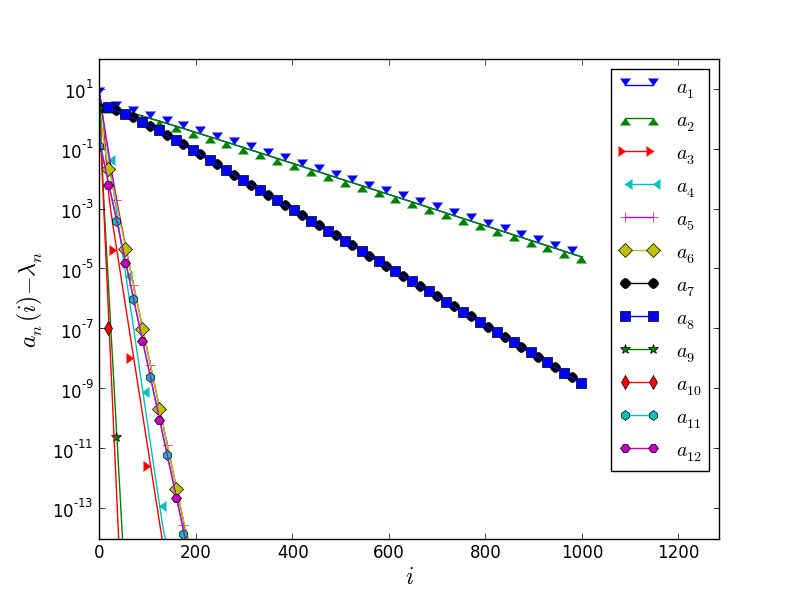
\includegraphics[height=7cm]{12x12randn_eigv_conv_QRstandard.png}
	\begin{scriptsize}
	\begin{tabular}{ll}
		\hline
		\hline
		\\
		$\lambda_1=
		-6.544395991691173
		$ & $\lambda_2=
		6.583845448270952
		$ \\ $\lambda_3=
		-4.759692498020273
		$ & $\lambda_4=
		4.227228411195598
		$ \\ $\lambda_5=
		-3.718806489258647
		$ & $\lambda_6=
		3.406092305333206
		$ \\ $\lambda_7=
		-2.508608861858869
		$ & $\lambda_8=
		2.480820818364306
		$ \\ $\lambda_9=
		-1.768319271480477
		$ & $\lambda_{10}=
		0.731101702075869
		$ \\ $\lambda_{11}=
		-0.4860591502185416
		$ & $\lambda_{12}=
		0.4459711429826421
		$ \\
		\\
		\hline
		\hline
	\end{tabular}
	\end{scriptsize}
\caption{
	The basic QR- algorithm without shifts. The convergence of the leading principal submatrix
	of dimension $k$ is $\propto |(\lambda_k/\lambda_{k+1})|^i$
}
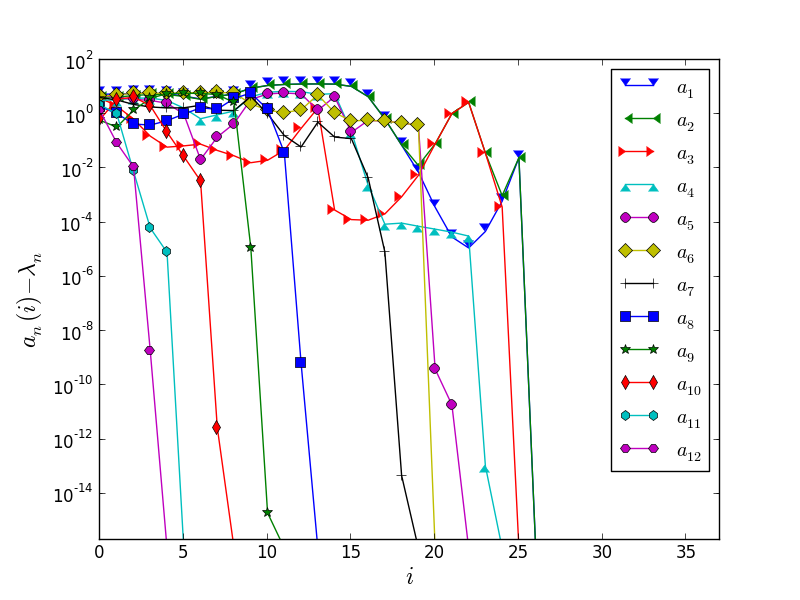
\includegraphics[height=7cm]{12x12randn_eigv_conv_QRfull.png}
	\begin{scriptsize}
	\begin{tabular}{ll}
		\hline
		\hline
		\\
		$\lambda_1=
		-6.544395991691173
		$ & $\lambda_2=
		6.583845448270952
		$ \\ $\lambda_3=
		-4.759692498020273
		$ & $\lambda_4=
		-3.718806489258647
		$ \\ $\lambda_5=
		2.480820818364306
		$ & $\lambda_6=
		4.227228411195598
		$ \\ $\lambda_7=
		3.406092305333206
		$ & $\lambda_8=
		-2.508608861858869
		$ \\ $\lambda_9=
		-1.768319271480477
		$ & $\lambda_{10}=
		-0.4860591502185416
		$ \\ $\lambda_{11}=
		0.731101702075869
		$ & $\lambda_{12}=
		0.4459711429826421
		$ \\
		\\
		\hline
		\hline
	\end{tabular}
	\end{scriptsize}
\caption{
	The full implicit QR- algorithm with Wilkinson shifts and deflation. Quadratic convergence
	of the shifted eigenvalue. 
}
\end{center}
\end{figure}%}}}3

\subsubsection*{Comparison with Lapack}

$1000\times1000$ real symmertic matrix with normal distributed random entries. 
My algo 20.69s, lapack 3.8s. $\approx$ 5 times speedup.

%}}}1

% vim:foldmethod=marker
